% CVPR 2027 submission: TempoRAC.  Template: cvpr-org/author-kit tag CVPR2027-v1
\documentclass[10pt,twocolumn,letterpaper]{article}
\usepackage[review]{cvpr}
\usepackage{caption}
\usepackage{booktabs}
\usepackage{multirow}
\usepackage{amsmath,amssymb}
\usepackage{bm}
\usepackage{xspace}
\usepackage{graphicx}
\usepackage{xr}
\usepackage{xcolor}
\usepackage{subcaption}
\usepackage{tikz}
\usetikzlibrary{arrows.meta,calc}

% user style: best values bold; improvements in dark red
\definecolor{darkred}{HTML}{B00000}
\newcommand{\imp}[1]{{\color{darkred}#1}}
\newcommand{\best}[1]{\textbf{#1}}
\newcommand{\method}{TempoRAC\xspace}
\newcommand{\TODO}[1]{\textbf{\color{red}[TODO: #1]}}
\DeclareMathOperator*{\argmax}{arg\,max}
\newcommand{\R}{\mathbb{R}}
% expandable input for generated table rows (LaTeX's \input breaks booktabs rules inside tabular)
\makeatletter\newcommand{\tabinput}[1]{\@@input #1.tex }\makeatother

\externaldocument{supplement}
\definecolor{cvprblue}{rgb}{0.21,0.49,0.74}
\usepackage[pagebackref,breaklinks,colorlinks,allcolors=cvprblue]{hyperref}

\def\confName{CVPR}
\def\confYear{2027}

\title{TempoRAC: Counting Repetitions at Every Tempo with a Multi-Rate Token Pyramid}

\author{Anonymous CVPR submission}

\begin{document}
\maketitle
\begin{abstract}
Repetition counting is dominated by tempo: cycles last from a fraction of a second
to several seconds and drift within a video, yet current counters observe every
video at a single temporal sampling rate, and the best rate depends on the tempo of
the repetition. We present \method, which reads a video at several tempi at once.
One frozen video transformer encodes the video at frame strides 2, 4 and 8 and at
two depths; overlapping clips are averaged into token streams aligned on a shared
frame grid, which are fused moment by moment and decoded into an event density
whose sum is the count. The shared grid gives the pyramid an exact property:
shifting it by one level yields the encoder output of the video played twice as
fast, a free tempo augmentation and a second test-time view. One decoder is trained
on the union of the public counting datasets with a dataset token and balanced
sampling. \TODO{headline RepCount-A numbers.}
\end{abstract}

% TempoRAC framework (TikZ). Included from main via % TempoRAC framework (TikZ). Included from main via % TempoRAC framework (TikZ). Included from main via \input{fig/framework}.
\begin{figure*}[t]
\centering
\resizebox{\textwidth}{!}{%
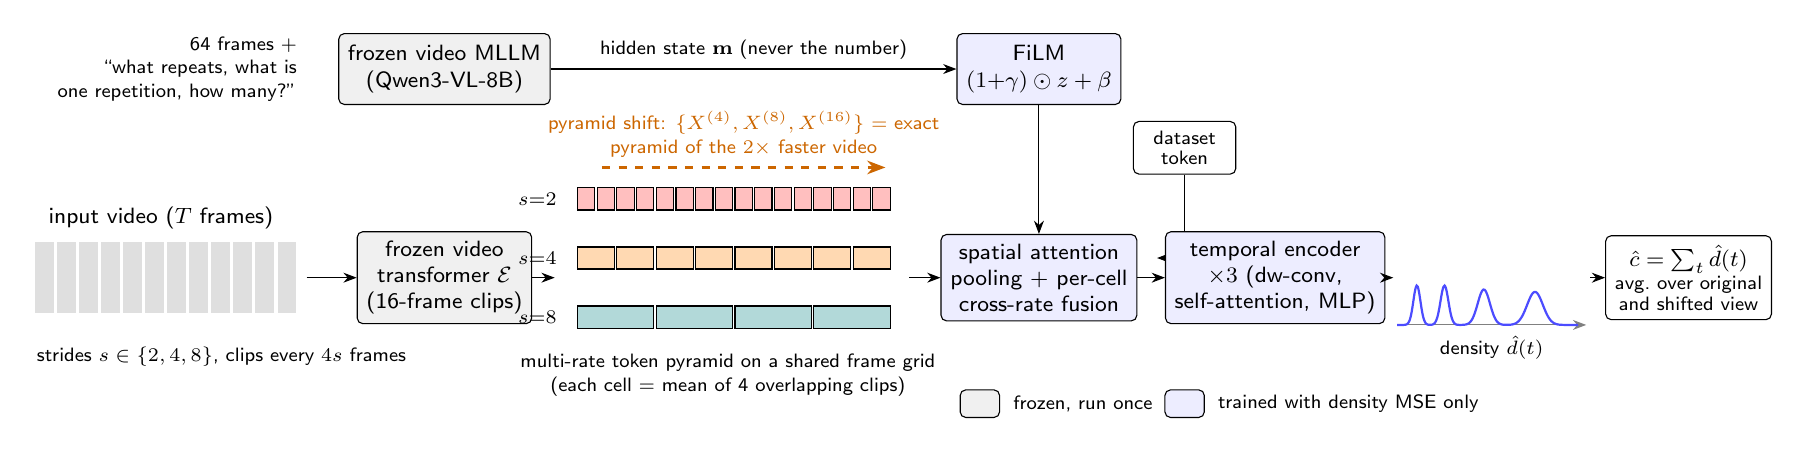
\begin{tikzpicture}[
  font=\sffamily\footnotesize, >=Stealth,
  box/.style={draw, rounded corners=2pt, minimum height=0.9cm, align=center, fill=white},
  frozen/.style={box, fill=gray!12},
  learn/.style={box, fill=blue!7},
  tok/.style={draw, minimum width=0.22cm, minimum height=0.28cm, inner sep=0pt},
]
% ---- input video
\foreach \i in {0,...,11} {
  \fill[gray!25] (\i*0.28, 0) rectangle ++(0.24, 0.9);
}
\node[anchor=south] at (1.6, 0.95) {input video ($T$ frames)};
% clip sampling rows
\foreach \s/\y/\c in {2/2.4/red!60, 4/1.6/orange!70, 8/0.8/teal!70} {}
\node[anchor=west, align=left] at (-0.1,-0.55) {\scriptsize strides $s\in\{2,4,8\}$, clips every $4s$ frames};
% ---- frozen encoder
\node[frozen, minimum width=2.1cm] (enc) at (5.2, 0.45) {frozen video\\transformer $\mathcal{E}$\\(16-frame clips)};
\draw[->] (3.45, 0.45) -- (enc.west);
% ---- token pyramid
\begin{scope}[shift={(7.0,-0.55)}]
  \foreach \k in {0,...,15} { \node[tok, fill=red!25]    at (\k*0.25, 2.0) {}; }
  \foreach \k in {0,...,7}  { \node[tok, fill=orange!30, minimum width=0.47cm] at (\k*0.5+0.125, 1.25) {}; }
  \foreach \k in {0,...,3}  { \node[tok, fill=teal!30, minimum width=0.97cm] at (\k*1.0+0.375, 0.5) {}; }
  \node[anchor=east] at (-0.25, 2.0) {\scriptsize $s{=}2$};
  \node[anchor=east] at (-0.25, 1.25) {\scriptsize $s{=}4$};
  \node[anchor=east] at (-0.25, 0.5) {\scriptsize $s{=}8$};
  \node[anchor=north, align=center] at (1.8, 0.15) {\scriptsize multi-rate token pyramid on a shared frame grid\\[-1pt]\scriptsize (each cell = mean of 4 overlapping clips)};
\end{scope}
\draw[->] (enc.east) -- (6.6, 0.45);
% ---- fusion
\node[learn, minimum width=1.9cm] (fuse) at (12.75, 0.45) {spatial attention\\pooling + per-cell\\cross-rate fusion};
\draw[->] (11.1, 0.45) -- (fuse.west);
% ---- semantic branch (frozen video MLLM -> FiLM) and dataset token
\node[frozen, minimum width=2.6cm] (mllm) at (5.2, 3.1) {frozen video MLLM\\(Qwen3-VL-8B)};
\node[anchor=east, align=right] at (3.45, 3.1) {\scriptsize 64 frames +\\[-1pt]\scriptsize ``what repeats, what is\\[-1pt]\scriptsize one repetition, how many?''};
\node[learn, minimum width=1.6cm] (film) at (12.75, 3.1) {FiLM\\$(1{+}\gamma)\odot z+\beta$};
\draw[->] (mllm.east) -- node[above] {\scriptsize hidden state $\mathbf{m}$ (never the number)} (film.west);
\draw[->] (film.south) -- (fuse.north);
\node[box, minimum width=1.3cm, minimum height=0.6cm] (tok) at (14.6, 2.1) {\scriptsize dataset\\[-2pt]\scriptsize token};
\draw[->] (tok.south) |- ($(fuse.east)+(0.25,0.25)$);
% ---- pyramid shift
\draw[->, dashed, thick, orange!80!black] (7.2, 1.85) -- node[above, align=center] {\scriptsize pyramid shift: $\{X^{(4)},X^{(8)},X^{(16)}\}$ = exact\\[-1pt]\scriptsize pyramid of the $2\times$ faster video} (10.8, 1.85);
% ---- temporal encoder
\node[learn, minimum width=1.8cm] (te) at (15.75, 0.45) {temporal encoder\\$\times3$ (dw-conv,\\self-attention, MLP)};
\draw[->] (fuse.east) -- (te.west);
% ---- density
\begin{scope}[shift={(17.3,-0.15)}]
  \draw[->, gray] (0,0) -- (2.4,0);
  \draw[thick, blue!70] plot[smooth, domain=0:2.3, samples=150] (\x, {0.5*exp(-(\x-0.25)*(\x-0.25)/0.004)+0.5*exp(-(\x-0.6)*(\x-0.6)/0.005)+0.45*exp(-(\x-1.1)*(\x-1.1)/0.012)+0.42*exp(-(\x-1.75)*(\x-1.75)/0.02)});
  \node[anchor=north] at (1.2, -0.02) {\scriptsize density $\hat d(t)$};
\end{scope}
\draw[->] (te.east) -- (17.25, 0.45);
\node[box, minimum width=1.3cm, align=center] (cnt) at (21.0, 0.45) {$\hat c=\sum_t \hat d(t)$\\[-1pt]\scriptsize avg.\ over original\\[-2pt]\scriptsize and shifted view};
\draw[->] (19.75, 0.45) -- (cnt.west);
% legend
\node[frozen, minimum height=0.35cm, minimum width=0.5cm] at (12.0, -1.15) {};
\node[anchor=west] at (12.3, -1.15) {\scriptsize frozen, run once};
\node[learn, minimum height=0.35cm, minimum width=0.5cm] at (14.6, -1.15) {};
\node[anchor=west] at (14.9, -1.15) {\scriptsize trained with density MSE only};
\end{tikzpicture}}
\caption{\method. A frozen video transformer reads the video at frame strides
2, 4 and 8 and at two depths; overlapping clips are averaged into token streams
on a shared frame grid, pooled over space, fused per cell, processed by a
temporal encoder and decoded once into an event density whose sum is the count.
A frozen video MLLM is asked what is repeated and what one repetition consists
of; its hidden state modulates the fused cells (FiLM), together with a learned
dataset token, so that one decoder can be trained on several datasets. Shifting
the pyramid by one level gives the exact tokens of the video played twice as
fast, used as training augmentation and as a second test-time view.}
\label{fig:framework}
\end{figure*}
.
\begin{figure*}[t]
\centering
\resizebox{\textwidth}{!}{%
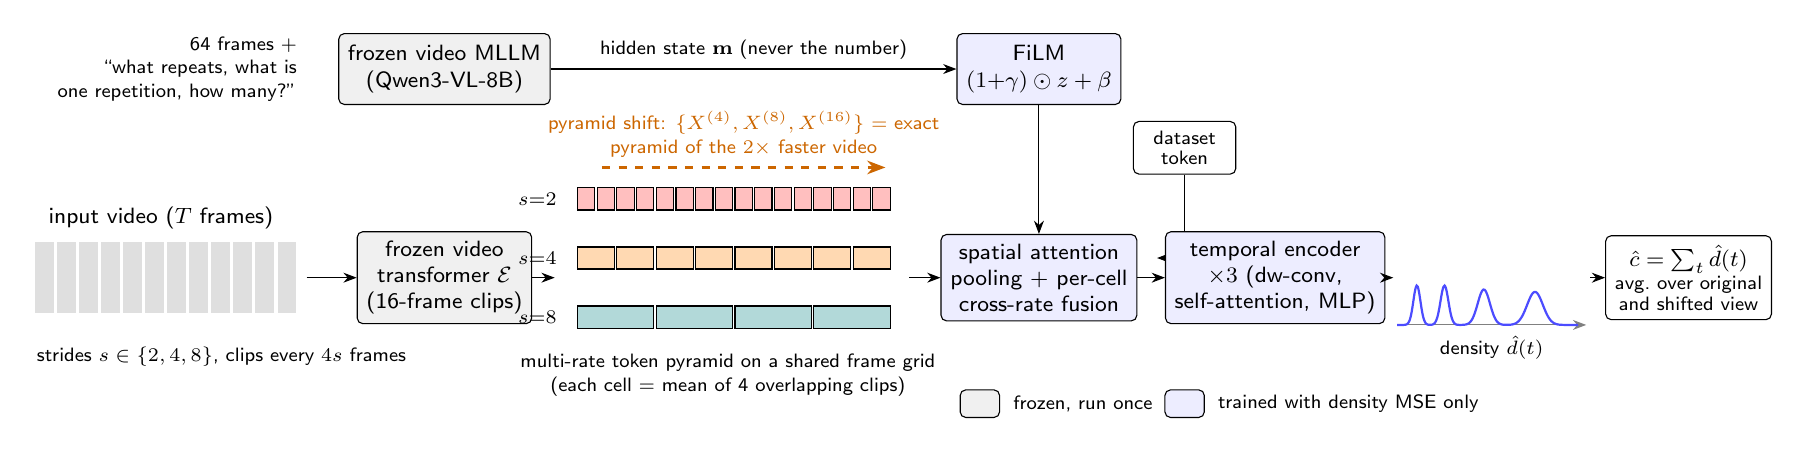
\begin{tikzpicture}[
  font=\sffamily\footnotesize, >=Stealth,
  box/.style={draw, rounded corners=2pt, minimum height=0.9cm, align=center, fill=white},
  frozen/.style={box, fill=gray!12},
  learn/.style={box, fill=blue!7},
  tok/.style={draw, minimum width=0.22cm, minimum height=0.28cm, inner sep=0pt},
]
% ---- input video
\foreach \i in {0,...,11} {
  \fill[gray!25] (\i*0.28, 0) rectangle ++(0.24, 0.9);
}
\node[anchor=south] at (1.6, 0.95) {input video ($T$ frames)};
% clip sampling rows
\foreach \s/\y/\c in {2/2.4/red!60, 4/1.6/orange!70, 8/0.8/teal!70} {}
\node[anchor=west, align=left] at (-0.1,-0.55) {\scriptsize strides $s\in\{2,4,8\}$, clips every $4s$ frames};
% ---- frozen encoder
\node[frozen, minimum width=2.1cm] (enc) at (5.2, 0.45) {frozen video\\transformer $\mathcal{E}$\\(16-frame clips)};
\draw[->] (3.45, 0.45) -- (enc.west);
% ---- token pyramid
\begin{scope}[shift={(7.0,-0.55)}]
  \foreach \k in {0,...,15} { \node[tok, fill=red!25]    at (\k*0.25, 2.0) {}; }
  \foreach \k in {0,...,7}  { \node[tok, fill=orange!30, minimum width=0.47cm] at (\k*0.5+0.125, 1.25) {}; }
  \foreach \k in {0,...,3}  { \node[tok, fill=teal!30, minimum width=0.97cm] at (\k*1.0+0.375, 0.5) {}; }
  \node[anchor=east] at (-0.25, 2.0) {\scriptsize $s{=}2$};
  \node[anchor=east] at (-0.25, 1.25) {\scriptsize $s{=}4$};
  \node[anchor=east] at (-0.25, 0.5) {\scriptsize $s{=}8$};
  \node[anchor=north, align=center] at (1.8, 0.15) {\scriptsize multi-rate token pyramid on a shared frame grid\\[-1pt]\scriptsize (each cell = mean of 4 overlapping clips)};
\end{scope}
\draw[->] (enc.east) -- (6.6, 0.45);
% ---- fusion
\node[learn, minimum width=1.9cm] (fuse) at (12.75, 0.45) {spatial attention\\pooling + per-cell\\cross-rate fusion};
\draw[->] (11.1, 0.45) -- (fuse.west);
% ---- semantic branch (frozen video MLLM -> FiLM) and dataset token
\node[frozen, minimum width=2.6cm] (mllm) at (5.2, 3.1) {frozen video MLLM\\(Qwen3-VL-8B)};
\node[anchor=east, align=right] at (3.45, 3.1) {\scriptsize 64 frames +\\[-1pt]\scriptsize ``what repeats, what is\\[-1pt]\scriptsize one repetition, how many?''};
\node[learn, minimum width=1.6cm] (film) at (12.75, 3.1) {FiLM\\$(1{+}\gamma)\odot z+\beta$};
\draw[->] (mllm.east) -- node[above] {\scriptsize hidden state $\mathbf{m}$ (never the number)} (film.west);
\draw[->] (film.south) -- (fuse.north);
\node[box, minimum width=1.3cm, minimum height=0.6cm] (tok) at (14.6, 2.1) {\scriptsize dataset\\[-2pt]\scriptsize token};
\draw[->] (tok.south) |- ($(fuse.east)+(0.25,0.25)$);
% ---- pyramid shift
\draw[->, dashed, thick, orange!80!black] (7.2, 1.85) -- node[above, align=center] {\scriptsize pyramid shift: $\{X^{(4)},X^{(8)},X^{(16)}\}$ = exact\\[-1pt]\scriptsize pyramid of the $2\times$ faster video} (10.8, 1.85);
% ---- temporal encoder
\node[learn, minimum width=1.8cm] (te) at (15.75, 0.45) {temporal encoder\\$\times3$ (dw-conv,\\self-attention, MLP)};
\draw[->] (fuse.east) -- (te.west);
% ---- density
\begin{scope}[shift={(17.3,-0.15)}]
  \draw[->, gray] (0,0) -- (2.4,0);
  \draw[thick, blue!70] plot[smooth, domain=0:2.3, samples=150] (\x, {0.5*exp(-(\x-0.25)*(\x-0.25)/0.004)+0.5*exp(-(\x-0.6)*(\x-0.6)/0.005)+0.45*exp(-(\x-1.1)*(\x-1.1)/0.012)+0.42*exp(-(\x-1.75)*(\x-1.75)/0.02)});
  \node[anchor=north] at (1.2, -0.02) {\scriptsize density $\hat d(t)$};
\end{scope}
\draw[->] (te.east) -- (17.25, 0.45);
\node[box, minimum width=1.3cm, align=center] (cnt) at (21.0, 0.45) {$\hat c=\sum_t \hat d(t)$\\[-1pt]\scriptsize avg.\ over original\\[-2pt]\scriptsize and shifted view};
\draw[->] (19.75, 0.45) -- (cnt.west);
% legend
\node[frozen, minimum height=0.35cm, minimum width=0.5cm] at (12.0, -1.15) {};
\node[anchor=west] at (12.3, -1.15) {\scriptsize frozen, run once};
\node[learn, minimum height=0.35cm, minimum width=0.5cm] at (14.6, -1.15) {};
\node[anchor=west] at (14.9, -1.15) {\scriptsize trained with density MSE only};
\end{tikzpicture}}
\caption{\method. A frozen video transformer reads the video at frame strides
2, 4 and 8 and at two depths; overlapping clips are averaged into token streams
on a shared frame grid, pooled over space, fused per cell, processed by a
temporal encoder and decoded once into an event density whose sum is the count.
A frozen video MLLM is asked what is repeated and what one repetition consists
of; its hidden state modulates the fused cells (FiLM), together with a learned
dataset token, so that one decoder can be trained on several datasets. Shifting
the pyramid by one level gives the exact tokens of the video played twice as
fast, used as training augmentation and as a second test-time view.}
\label{fig:framework}
\end{figure*}
.
\begin{figure*}[t]
\centering
\resizebox{\textwidth}{!}{%
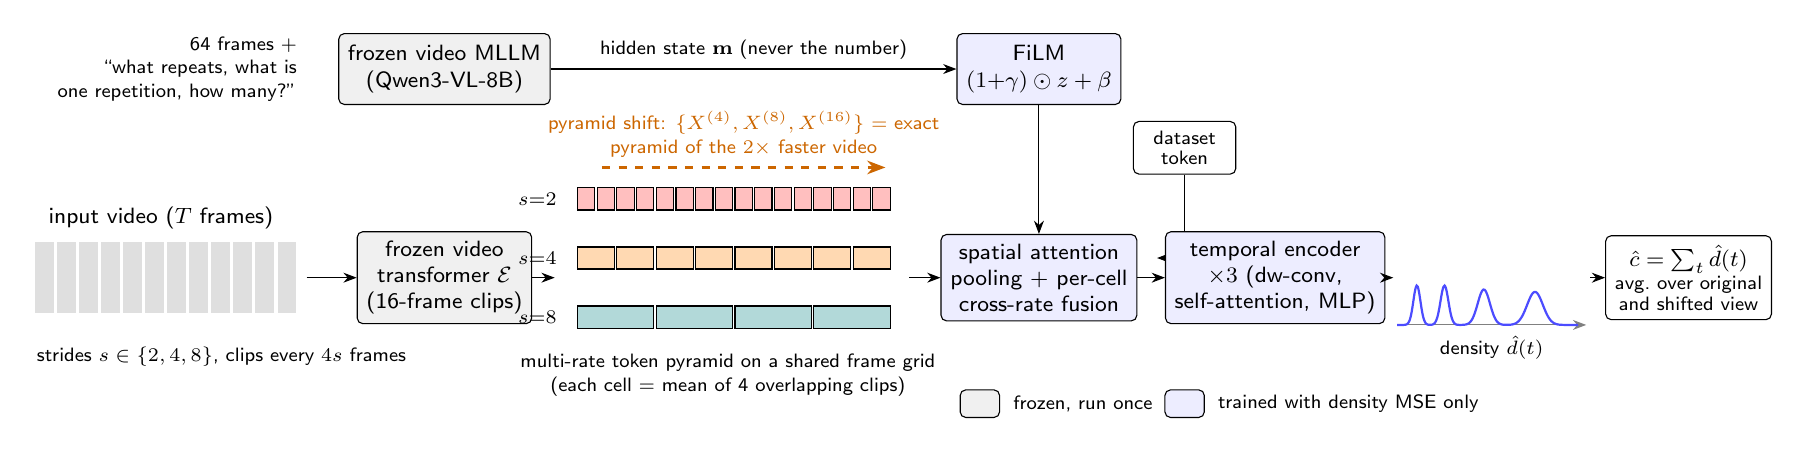
\begin{tikzpicture}[
  font=\sffamily\footnotesize, >=Stealth,
  box/.style={draw, rounded corners=2pt, minimum height=0.9cm, align=center, fill=white},
  frozen/.style={box, fill=gray!12},
  learn/.style={box, fill=blue!7},
  tok/.style={draw, minimum width=0.22cm, minimum height=0.28cm, inner sep=0pt},
]
% ---- input video
\foreach \i in {0,...,11} {
  \fill[gray!25] (\i*0.28, 0) rectangle ++(0.24, 0.9);
}
\node[anchor=south] at (1.6, 0.95) {input video ($T$ frames)};
% clip sampling rows
\foreach \s/\y/\c in {2/2.4/red!60, 4/1.6/orange!70, 8/0.8/teal!70} {}
\node[anchor=west, align=left] at (-0.1,-0.55) {\scriptsize strides $s\in\{2,4,8\}$, clips every $4s$ frames};
% ---- frozen encoder
\node[frozen, minimum width=2.1cm] (enc) at (5.2, 0.45) {frozen video\\transformer $\mathcal{E}$\\(16-frame clips)};
\draw[->] (3.45, 0.45) -- (enc.west);
% ---- token pyramid
\begin{scope}[shift={(7.0,-0.55)}]
  \foreach \k in {0,...,15} { \node[tok, fill=red!25]    at (\k*0.25, 2.0) {}; }
  \foreach \k in {0,...,7}  { \node[tok, fill=orange!30, minimum width=0.47cm] at (\k*0.5+0.125, 1.25) {}; }
  \foreach \k in {0,...,3}  { \node[tok, fill=teal!30, minimum width=0.97cm] at (\k*1.0+0.375, 0.5) {}; }
  \node[anchor=east] at (-0.25, 2.0) {\scriptsize $s{=}2$};
  \node[anchor=east] at (-0.25, 1.25) {\scriptsize $s{=}4$};
  \node[anchor=east] at (-0.25, 0.5) {\scriptsize $s{=}8$};
  \node[anchor=north, align=center] at (1.8, 0.15) {\scriptsize multi-rate token pyramid on a shared frame grid\\[-1pt]\scriptsize (each cell = mean of 4 overlapping clips)};
\end{scope}
\draw[->] (enc.east) -- (6.6, 0.45);
% ---- fusion
\node[learn, minimum width=1.9cm] (fuse) at (12.75, 0.45) {spatial attention\\pooling + per-cell\\cross-rate fusion};
\draw[->] (11.1, 0.45) -- (fuse.west);
% ---- semantic branch (frozen video MLLM -> FiLM) and dataset token
\node[frozen, minimum width=2.6cm] (mllm) at (5.2, 3.1) {frozen video MLLM\\(Qwen3-VL-8B)};
\node[anchor=east, align=right] at (3.45, 3.1) {\scriptsize 64 frames +\\[-1pt]\scriptsize ``what repeats, what is\\[-1pt]\scriptsize one repetition, how many?''};
\node[learn, minimum width=1.6cm] (film) at (12.75, 3.1) {FiLM\\$(1{+}\gamma)\odot z+\beta$};
\draw[->] (mllm.east) -- node[above] {\scriptsize hidden state $\mathbf{m}$ (never the number)} (film.west);
\draw[->] (film.south) -- (fuse.north);
\node[box, minimum width=1.3cm, minimum height=0.6cm] (tok) at (14.6, 2.1) {\scriptsize dataset\\[-2pt]\scriptsize token};
\draw[->] (tok.south) |- ($(fuse.east)+(0.25,0.25)$);
% ---- pyramid shift
\draw[->, dashed, thick, orange!80!black] (7.2, 1.85) -- node[above, align=center] {\scriptsize pyramid shift: $\{X^{(4)},X^{(8)},X^{(16)}\}$ = exact\\[-1pt]\scriptsize pyramid of the $2\times$ faster video} (10.8, 1.85);
% ---- temporal encoder
\node[learn, minimum width=1.8cm] (te) at (15.75, 0.45) {temporal encoder\\$\times3$ (dw-conv,\\self-attention, MLP)};
\draw[->] (fuse.east) -- (te.west);
% ---- density
\begin{scope}[shift={(17.3,-0.15)}]
  \draw[->, gray] (0,0) -- (2.4,0);
  \draw[thick, blue!70] plot[smooth, domain=0:2.3, samples=150] (\x, {0.5*exp(-(\x-0.25)*(\x-0.25)/0.004)+0.5*exp(-(\x-0.6)*(\x-0.6)/0.005)+0.45*exp(-(\x-1.1)*(\x-1.1)/0.012)+0.42*exp(-(\x-1.75)*(\x-1.75)/0.02)});
  \node[anchor=north] at (1.2, -0.02) {\scriptsize density $\hat d(t)$};
\end{scope}
\draw[->] (te.east) -- (17.25, 0.45);
\node[box, minimum width=1.3cm, align=center] (cnt) at (21.0, 0.45) {$\hat c=\sum_t \hat d(t)$\\[-1pt]\scriptsize avg.\ over original\\[-2pt]\scriptsize and shifted view};
\draw[->] (19.75, 0.45) -- (cnt.west);
% legend
\node[frozen, minimum height=0.35cm, minimum width=0.5cm] at (12.0, -1.15) {};
\node[anchor=west] at (12.3, -1.15) {\scriptsize frozen, run once};
\node[learn, minimum height=0.35cm, minimum width=0.5cm] at (14.6, -1.15) {};
\node[anchor=west] at (14.9, -1.15) {\scriptsize trained with density MSE only};
\end{tikzpicture}}
\caption{\method. A frozen video transformer reads the video at frame strides
2, 4 and 8 and at two depths; overlapping clips are averaged into token streams
on a shared frame grid, pooled over space, fused per cell, processed by a
temporal encoder and decoded once into an event density whose sum is the count.
A frozen video MLLM is asked what is repeated and what one repetition consists
of; its hidden state modulates the fused cells (FiLM), together with a learned
dataset token, so that one decoder can be trained on several datasets. Shifting
the pyramid by one level gives the exact tokens of the video played twice as
fast, used as training augmentation and as a second test-time view.}
\label{fig:framework}
\end{figure*}

\section{Introduction}
\label{sec:intro}

Counting how many times an action repeats---push-ups in a workout, strokes of a
saw, turns of a wheel---is a basic form of temporal understanding with uses in
fitness, rehabilitation and industrial monitoring. It needs two abilities that
are rarely found in one model. The first is \emph{temporal precision at every
tempo}: on RepCount-A~\cite{hu2022transrac} the median cycle of a video ranges
from 0.85\,s to 4.75\,s (5th--95th percentile), and in one video out of five the
cycle length varies by more than 25\% as people accelerate, tire or pause. The
second is \emph{knowing what one repetition is}: a push-up is a down- and an
up-stroke, a cello bow stroke is one back-and-forth. The visual signal of many
actions repeats every half cycle, and which period counts is a convention of the
action, not a property of the motion.

Dedicated counters have the first ability and lack the second. They regress a
density or a period from video features at one temporal sampling rate, and their
largest errors are counts that are off by a factor of about two on symmetric
motions (\cref{sec:analysis}). Video multimodal large language models (MLLMs)
have the second ability and lack the first: asked how often an action repeats, a
recent 8B MLLM names the action and describes one repetition correctly, but its
counts are far off (zero-shot MAE 0.43--0.55 on four benchmarks). CountLLM~\cite{yao2025countllm}
fine-tunes an LLM to output the count as text, which ties both abilities to the
language model.

We present \method, a counter that takes temporal precision from a frozen
video encoder and semantics from a frozen MLLM. A \emph{multi-rate token
pyramid} encodes the video at three frame strides and two depths of the encoder
on a shared frame grid, and a decoder turns it into an event density whose sum is
the count. A frozen video MLLM reads the video once, is asked what is repeated
and what one repetition consists of, and its hidden state modulates the decoder;
the MLLM is never asked for the number. Two properties follow from this design.
First, because all pyramid levels live on one grid with stride-proportional clip
hops, \emph{shifting the pyramid by one level gives the exact encoder output of
the video played twice as fast}: tempo augmentation and a second test-time view
come for free, without re-encoding. Second, semantic conditioning lets one
counter learn from several datasets at once. Training on the union of
RepCount-A, Countix and UCFRep fails for an unconditioned counter---it improves
UCFRep but degrades RepCount-A, whose counting conventions are overridden by the
much larger Countix---and works once the decoder is told what is being repeated,
together with a learned dataset token and balanced sampling.

\TODO{results summary: RepCount-A, UCFRep, Countix test; QUVA zero-shot.}

Our contributions are:
\begin{itemize}
  \setlength\itemsep{0pt}
  \setlength\parskip{0pt}
  \item A division of labour for repetition counting in which a frozen video MLLM
  supplies what to count and a density decoder on a multi-rate token pyramid
  supplies how many, with an analysis of why each alone falls short.
  \item The pyramid-shift property, which turns the token pyramid into exact
  tempo-changed views for training and inference at no encoding cost.
  \item Semantically conditioned joint training across RAC datasets, with
  component ablations over five seeds and state-of-the-art results \TODO{claim
  after test runs}; code, splits, features and per-video predictions will be
  released.
\end{itemize}

\section{Related Work}
\label{sec:related}

\paragraph{Repetition counting.}
Early approaches estimated a dominant frequency from motion signals or learned
live counters on short periodic clips~\cite{levy2015live,runia2018realworld}.
RepNet~\cite{dwibedi2020repnet} introduced the temporal self-similarity matrix
(TSM) as a class-agnostic bottleneck and predicts a per-frame period length and
periodicity. Zhang~\etal~\cite{zhang2020context} predict the lengths of the
cycles around each frame and resample the video around them in a coarse-to-fine
manner, and Sight\&Sound~\cite{zhang2021sight} adds audio. TransRAC~\cite{hu2022transrac}
released RepCount, with fine-grained cycle annotations and large period
variation, and regresses a density from multi-scale TSMs. Later methods improved
motion features~\cite{li2024mfl}, resolution~\cite{li2023fullres}, query
design~\cite{ma2026detrc} and dual-branch spatio-temporal
attention~\cite{wang2026d2stx}. ESCounts~\cite{sinha2024escounts} trains a
decoder on frozen masked-autoencoder video tokens with repetition exemplars and
counts exemplar-free at test time. Pose-based counters exploit salient body
poses~\cite{yao2025poserac} or period-adaptive
self-supervision~\cite{gao2026pams}; CountLLM~\cite{yao2025countllm} leverages
a large language model and web-scale video--text pre-training.

\paragraph{Tempo and sampling rate.}
Most counters fix the temporal sampling of their input: TransRAC resamples every
video to 64 frames, ESCounts encodes clips with one frame stride (it compares
strides 4 to 32 one at a time and finds denser sampling better).
RepNet~\cite{dwibedi2020repnet} scans several speeds at test time and keeps the
one with the most confident periodicity; Sight\&Sound learns to choose one
stride per video; Zhang~\etal~\cite{zhang2020context} adapt the sampling window
to predicted cycle lengths. All of these commit to one rate per video or per
window. Closest to us, multi-stride collaboration~\cite{gan2023multistride}
counts a video at several strides and combines the resulting counts. \method
instead fuses the token streams of all strides at every moment, before any
temporal reasoning, and we show that committing to a rate---even one chosen by a
supervised tempo estimator---is worse than letting the decoder see all of them.

\paragraph{Multi-rate video models.}
Two-pathway models such as SlowFast~\cite{feichtenhofer2019slowfast} combine a
low and a high frame rate with separately trained pathways and lateral
connections. Our pyramid uses a single frozen encoder at several strides and
aligns the streams on a common frame grid, which keeps the encoder run once per
video and stride and makes the fusion a per-cell operation.

\section{TempoRAC}
\label{sec:method}

Given a video of $T$ frames, a counter predicts a non-negative event density
$\hat d(t)$ on a fine temporal grid whose sum is the repetition count,
$\hat c=\sum_t\hat d(t)$. \method (\cref{fig:framework}) combines the two
abilities that counting needs. \emph{Temporal precision at every tempo} comes
from a multi-rate token pyramid of a count-adapted video encoder, read at two
depths (\cref{sec:pyramid,sec:adapt}) and decoded into a density
(\cref{sec:decoder}); the pyramid yields exact tempo-changed views of a video
for free (\cref{sec:shift}), and one decoder is trained on several datasets
(\cref{sec:joint}). \emph{Knowing what is repeated} enters where the decoder
needs it: each exact view is reliable in a different tempo range, and a
frozen MLLM's description of the action indexes a memory of held-out outcomes
that decides how much to trust each view (\cref{sec:llm}); the reported count is
always a weighted sum of density integrals.

\subsection{Multi-rate, two-depth token pyramid}
\label{sec:pyramid}
A frozen video transformer $\mathcal{E}$ maps a clip of 16 frames to
$8\times H\times W$ tokens; each temporal token summarises two consecutive input
frames (tubelet size 2). For a frame stride $s$ the clip spans $16s$ frames of
the video and one token covers $2s$ frames. We use strides
$\mathcal{S}=\{2,4,8\}$, so the pyramid's clips span roughly 1, 2 and 4 seconds
at 30\,fps and its tokens cover 4, 8 and 16 frames. The fine level resolves
fast repetitions; the coarse level sees two to four slow cycles inside a single
clip (\cref{sec:observation}). All levels use the same encoder and
pre-processing, so they differ only in temporal sampling.

\paragraph{Dense, grid-aligned encoding.}
For each stride we start a clip every $4s$ frames. A clip starting at frame $j$
contributes its $k$-th temporal token to grid cell $j/2s+k$ of a stride-specific
grid with $\lceil T/2s\rceil$ cells of $2s$ frames, so every cell is seen by
four overlapping clips with different temporal context; we average their tokens.
Each stream thus becomes a regular sequence on a known frame grid, which is what
allows streams of different strides to be fused cell by cell and, as shown in
\cref{sec:shift}, to be exchanged exactly. Spatial tokens are average-pooled to
$4\times4$ and stored, so the encoder runs once per video and stride.

\paragraph{Two depths.}
The last block of a masked-autoencoder encoder is shaped by pixel
reconstruction, and intermediate blocks of such encoders transfer better when
frozen. We read every clip after block 8 and after the final block 12 (the
former standardised without learned affine parameters) and concatenate the two
token sets channel-wise in every cell.

\subsection{Count-aware encoder adaptation}
\label{sec:adapt}
A frozen self-supervised encoder is not tuned to periodic motion: counters that
fine-tune their encoder are far stronger on UCFRep than those that keep it
frozen~\cite{zhang2020context,sinha2024escounts}, and in CountLLM adapting the
video encoder is the largest single gain~\cite{yao2025countllm}. Back-propagating
through the whole overlapping pyramid is too expensive, so we adapt the encoder
once, before the pyramid is extracted. From every training video we sample a
window of four non-overlapping 16-frame clips at a stride drawn from
$\{2,4,8\}$, so that every pyramid level is adapted, and train LoRA
factors~\cite{hu2022lora} (rank 8) on the query, key, value and output
projections of all twelve blocks together with a small counting head
(attention pooling over space and a two-layer temporal transformer) that predicts,
for every temporal token, the integral of the target density over its $2s$
frames. The epoch is selected on validation windows; the LoRA factors are then
merged into the encoder, which re-encodes the full pyramid of every video.

\subsection{Counting decoder}
\label{sec:decoder}
Each stream $\mathbf{X}^{(s)}\in\R^{T_s\times 16\times C}$ is reduced over space
by attention pooling---a layer norm, a projection to width $D$, and a softmax
over the 16 spatial positions of a learned scoring MLP---giving
$\mathbf{x}^{(s)}_t\in\R^D$. Streams are brought to the finest grid by
repeating every coarse cell $s/2$ times and fused per cell by a linear map,
$\mathbf{z}_t=W[\mathbf{x}^{(2)}_t\Vert\mathbf{x}^{(4)}_t\Vert\mathbf{x}^{(8)}_t]$.
A temporal encoder of three pre-norm blocks---a depthwise temporal convolution (kernel 5) for local motion,
multi-head self-attention for cycle-to-cycle comparisons, and an MLP---processes
the whole video with sinusoidal positions measured in frames, and a two-layer
head with a softplus output gives $\hat d$ on a grid of 2-frame cells. The
density of the whole video is predicted in one pass and summed once, so no window
is counted on its own and no boundary reconciliation is needed.

\paragraph{Objective.}
For each annotated cycle $[a_k,b_k]$ we place a Gaussian at $(a_k+b_k)/2$ with
standard deviation $(b_k-a_k)/4$, normalised to unit mass on the cell grid
(cycles cut by a training crop keep their partial mass), and sum them into a
target $y(t)$ with $\sum_t y(t)=c$. For datasets that only provide a count over
a segment, cycles are placed uniformly over the segment, as in
ESCounts~\cite{sinha2024escounts}. The loss is the density error alone,
\begin{equation}
\mathcal{L}=\frac{1}{T'}\sum_{t}\big(\hat d(t)-y(t)\big)^2 ,
\label{eq:loss}
\end{equation}
averaged over the $T'$ valid cells of a video.

\subsection{Pyramid shift: exact tempo changes for free}
\label{sec:shift}
Because all levels share one frame grid and their clip hops and token widths
scale with the stride, the pyramid has a simple algebraic property.
\begin{quote}\itshape
Let $V'$ be $V$ played twice as fast, $V'[i]=V[2i]$. The stride-$s$ stream of
$V'$ equals the stride-$2s$ stream of $V$.
\end{quote}
A stride-$s$ clip of $V'$ starting at frame $j$ reads $V'[j+sf]=V[2j+2sf]$,
$f=0,\dots,15$, which is the stride-$2s$ clip of $V$ starting at $2j$; clips of
$V'$ start every $4s$ frames, i.e.\ every $8s$ frames of $V$, which are exactly
the stride-$2s$ starts; and a stride-$s$ cell of $V'$ covers $2s$ frames of
$V'$, i.e.\ $4s$ frames of $V$, a stride-$2s$ cell. Hence shifting the pyramid one
level up, $\{\mathbf{X}^{(2)},\mathbf{X}^{(4)},\mathbf{X}^{(8)}\}\leftarrow
\{\mathbf{X}^{(4)},\mathbf{X}^{(8)},\mathbf{X}^{(16)}\}$, yields the exact
encoder output of the accelerated video, with no re-encoding and no
interpolation of features; cycle boundaries halve and the count is unchanged.
This costs one extra coarse level ($s{=}16$, one clip every 64 frames).

\paragraph{Training.} With probability $0.5$ a training video (after cropping) is
replaced by its shifted pyramid. Acceleration is only applied when every cycle
stays at least 8 frames long after it, so that the finest stream still samples
each cycle in at least two cells; otherwise the shifted view would be aliased
and its label unlearnable. The augmentation adds the fast tempi that are rare in
training data and on which counters under-count (\cref{sec:analysis}).

\paragraph{Inference.} The count of a video does not depend on its playback
speed, so the shifted pyramid is a second, exactly computed view of every test
video. We report the average of the counts predicted from the two views; model
selection uses the original view only.

\subsection{Counting across datasets}
\label{sec:joint}
Public RAC datasets are small (RepCount-A has 758 training videos, UCFRep 421)
and annotate different actions with different conventions. Training one counter
on their union is attractive, but naively the union is dominated by the 4{,}224
short Countix clips and the counter's count prior shifts towards them, so that
RepCount-A under-counts its long videos. Two pieces make joint training work.
A learned \emph{dataset token}, one $D$-dimensional vector per
source dataset initialised at zero, is added to every fused cell, so that
residual differences in annotation conventions need not be resolved by the
shared weights. \emph{Balanced sampling} repeats every RepCount-A and UCFRep
training video four times per epoch, so that Countix provides less than half of
the updates; we train for 50 epochs, which keeps the number of updates equal to
80 epochs without repetition. A single training run serves all three
benchmarks: we keep, for each dataset, the checkpoint that is best on its own
validation split and evaluate it once on its test split.

\subsection{Choosing the tempo by what is repeated}
\label{sec:llm}
The two views count the same video at two tempi, and each is right in a
different range: on the original view the decoder over-counts slow repetitions,
typically counting half-cycles, and on the $2\times$ view it under-counts fast
ones (\cref{sec:analysis}). Which view to trust cannot be read from the counts
themselves---the tempo a count implies is biased in the same direction as its
error---but it depends strongly on the action: on held-out videos, the view that
is right for one video of an action tends to be right for the others
(\cref{sec:analysis}). We therefore let a description of the action decide.

\paragraph{Describing the action.} A frozen Qwen3-VL-8B~\cite{qwen3vl} reads 64
frames of the counting span once and describes the repeated action and what one
repetition consists of (``action: push-up; one repetition: lower the body and
push back up''); the number it states is discarded. The description is embedded
with a sentence encoder (BGE-base~\cite{xiao2023cpack}).

\paragraph{A memory of held-out outcomes.} The memory holds, for every held-out
video $j$, its description embedding $\mathbf{e}_j$, which view was right
($y_{jk}{=}1$ for the view with the smallest normalised error $\epsilon_{jk}$,
split on ties) and how much the choice mattered,
$s_j=|\epsilon_{j,1\times}-\epsilon_{j,2\times}|$. For a new video with
embedding $\mathbf{e}$, the weight of view $k$ is the stake-weighted vote of its
$n$ nearest memory entries $\mathcal{N}$ in cosine similarity,
\begin{equation}
w_k=\frac{\sum_{j\in\mathcal{N}}s_j\,y_{jk}}{\sum_{j\in\mathcal{N}}s_j},\qquad
\hat c=\sum_k w_k\,\hat c_k ,
\label{eq:memory}
\end{equation}
so the count remains a weighted sum of density integrals and language decides only
the weights.

\paragraph{Held-out outcomes.} The outcomes must come from videos the decoder did
not train on: on its own training videos it is right in every view, which is also
why a language model that refines the converged decoder on those videos does not
help (\cref{tab:ablation}). As in blending~\cite{wolpert1992stacked}, the memory
holds the five decoders' predictions for the validation videos. Every validation
number of the selection is five-fold cross-validated over validation videos (folds
never split a source video, \eg a UCF101 group or a YouTube video); the number of
neighbours ($n{=}32$) and the embedded text (the whole description) are chosen by
cross-validation, and at test time the memory holds all validation videos; the
test splits are used once. Out-of-fold predictions on the training union, from
five cross-fitted decoders, are a worse memory, because on Countix the decoders err
differently on training and on validation clips (\cref{sec:analysis}).

\section{Experiments}
\label{sec:experiments}

\subsection{Setup}
\paragraph{Datasets.}
\textbf{RepCount-A}~\cite{hu2022transrac} contains 1{,}041 videos of fitness
and daily activities with per-cycle start/end annotations, split into
758/131/152 train/validation/test videos. Median cycle lengths range from
0.85\,s to 4.75\,s (5th--95th percentile of per-video medians), and 20\% of the
videos vary their cycle length by more than 25\%.
\textbf{UCFRep}~\cite{zhang2020context} annotates 526 UCF101 videos with cycle
boundaries (421/105 split); following Context and ESCounts we count inside the
annotated repetitive segment. Because UCF101 clips of one group are cut from the
same source video, model selection uses a development split of the 421 training
videos made of whole groups (331/90). We do not retrain on the 90 held-out
videos, so \method uses fewer UCFRep training videos than prior work.
\textbf{Countix}~\cite{dwibedi2020repnet} consists of Kinetics clips with counts.
We use the train/val/test split of ESCounts and retrieve 98\% of its videos
(4{,}224/1{,}374/2{,}403); exclusions (unresolvable or missing clips, exact
duplicate rows) are listed in the supplement. Countix has no cycle boundaries,
so density targets place the counted cycles uniformly over the repetition span,
as in ESCounts.
\textbf{QUVA}~\cite{runia2018realworld} (100 videos) is used only for zero-shot
evaluation of RepCount-A models. We verified every count and boundary against an
independent copy of the official annotations (zero mismatches on RepCount-A and
UCFRep).

\paragraph{Metrics and protocol.}
We report the normalised error
$\mathrm{MAE}=\frac{1}{N}\sum_i |\mathrm{round}(\hat c_i)-c_i|/(c_i+0.1)$ and
the off-by-one accuracy
$\mathrm{OBO}=\frac{1}{N}\sum_i\mathbb{1}[|\mathrm{round}(\hat c_i)-c_i|\le1]$
over videos with a positive count, exactly as in the released ESCounts
evaluation code; with this protocol the released ESCounts checkpoint obtains
0.215/0.556 on RepCount-A test in our pipeline, against its published
0.213/0.563. One training run on the union of the three training sets yields one
model per benchmark, selected on that benchmark's validation split (UCFRep: on
the development split) and evaluated once on its test split; no test video is
used for training or selection. We train five seeds (ablations: three) and
report mean$\pm$standard deviation; differences are tested with a paired
video-level bootstrap.

\paragraph{Implementation.}
The video encoder is the frozen ST-MAE ViT-B/16~\cite{feichtenhofer2022masked}
(Kinetics-400 self-supervised; the encoder of ESCounts), with shorter side 224, a
centre crop and ImageNet normalisation; tokens are taken after blocks 8 and 12.
The MLLM is Qwen3-VL-8B-Instruct~\cite{qwen3vl} in bf16, frozen, run once per
video with greedy decoding of at most 48 tokens. The decoder has width 256 and
6.1M trainable parameters; we use AdamW (learning rate $2\times10^{-4}$, weight
decay 0.05, cosine schedule with 3 warm-up epochs), batches of 8 whole videos,
50 epochs over the balanced union, random temporal crops covering at least 60\%
of a video with probability 0.5, pyramid shift with probability 0.5, and bf16
mixed precision. All experiments run on two RTX 4090 GPUs; caching the MLLM
outputs for all 9.8k videos takes about 2.7 hours, and one training run about
2 hours.

\subsection{Comparison with the state of the art}
\Cref{tab:main} \TODO{results discussion}.

\subsection{Ablations}
\Cref{tab:ablation} \TODO{ablation discussion: pyramid, overlap averaging,
objective, depth}.

\subsection{Generalisation and robustness}
\TODO{QUVA zero-shot, RepCount$\to$UCFRep/Countix, tempo-warp stress test.}

% Main comparison against external methods only. Published rows are the authors' own numbers
% (see docs/LITERATURE_NUMBERS_20261108.md); cross-dataset-only numbers are excluded from in-domain
% columns. PAMS Countix (0.098/0.879) is the authors' Table 1; docs/CITATION_AUDIT_20261109.md: subset and
% MAE normalisation unspecified, unnormalised MAE inconsistent with its OBO (>= 0.242 implied), no code.
\begin{table*}[t]
\centering
\caption{Comparison on RepCount-A (test), UCFRep (official val, used as test) and Countix (test).
MAE$\downarrow$, OBO$\uparrow$. Input: V = RGB video, P = pose, A = audio, F = optical flow,
L = large language model (CountLLM: fine-tuned after web-scale video--text alignment; \method: frozen,
never outputs the count). $\ddagger$: released checkpoint evaluated by us with the same protocol.
$\S$: trained on an 8-class, 487-video subset of RepCount-A.
$\P$: skeleton-only; the Countix videos used and the normalisation of MAE are not specified by the authors
(the paper's MAE definition is unnormalised, which its OBO value rules out), so this entry is not like-for-like.
\method: mean$\pm$std over 5 seeds of one jointly trained model per seed, two-view average; UCFRep uses 331 of
the 421 training videos. Best in bold; \imp{red}: improvement of \method over CountLLM, the strongest method
with the same input.}
\label{tab:main}
\small
\setlength{\tabcolsep}{4pt}
\begin{tabular}{llcccccc}
\toprule
& & \multicolumn{2}{c}{RepCount-A} & \multicolumn{2}{c}{UCFRep} & \multicolumn{2}{c}{Countix}\\
\cmidrule(lr){3-4}\cmidrule(lr){5-6}\cmidrule(lr){7-8}
Method & Input & MAE & OBO & MAE & OBO & MAE & OBO\\
\midrule
RepNet~\cite{dwibedi2020repnet} & V & 0.995 & 0.013 & -- & -- & 0.364 & 0.697\\
Context~\cite{zhang2020context} & V & 0.879 & 0.155 & 0.147 & 0.790 & -- & --\\
Sight\&Sound~\cite{zhang2021sight} & V(+A) & -- & -- & 0.143 & 0.800 & 0.307 & 0.511\\
TransRAC~\cite{hu2022transrac} & V & 0.443 & 0.291 & -- & -- & -- & --\\
MFL~\cite{li2024mfl} & V+F & 0.384 & 0.386 & 0.388 & 0.510 & -- & --\\
Full-Res~\cite{li2023fullres} & V & 0.410 & 0.327 & -- & -- & -- & --\\
DeTRC~\cite{ma2026detrc} & V & 0.262 & 0.543 & -- & -- & -- & --\\
D$^2$-STX~\cite{wang2026d2stx} & V+P & 0.255 & 0.500 & 0.236 & 0.777 & 0.278 & 0.734\\
ESCounts~\cite{sinha2024escounts} & V & 0.213 & 0.563 & 0.216 & 0.704 & 0.276 & 0.673\\
ESCounts$^\ddagger$ & V & 0.215 & 0.556 & -- & -- & -- & --\\
\midrule
PoseRAC~\cite{yao2025poserac}$^\S$ & P & 0.236 & 0.560 & -- & -- & -- & --\\
PAMS~\cite{gao2026pams}$^\P$ & P & \best{0.129} & \best{0.842} & 0.208 & 0.686 & \best{0.098} & \best{0.879}\\
\midrule
CountLLM~\cite{yao2025countllm} & V+L & 0.162 & 0.639 & \best{0.116} & \best{0.839} & 0.215 & 0.801\\
% numbers: runs/final_v2/main_table_numbers.json (full_s0..s4, test_tta)
\method (ours) & V+L & 0.142{\scriptsize$\pm$0.006} & 0.721{\scriptsize$\pm$0.019} & 0.206{\scriptsize$\pm$0.008} & 0.695{\scriptsize$\pm$0.020} & 0.238{\scriptsize$\pm$0.024} & 0.692{\scriptsize$\pm$0.035}\\
& & \imp{$-$12.3\%} & \imp{+0.082} & & & & \\
\bottomrule
\end{tabular}
\end{table*}

% Component ablations on RepCount-A (test); each model scored once. Rows written by
% temporac_cvpr/final_tables_frozen.py; all three benchmarks in the appendix (tab:app_ablation).
\begin{table}[t]
\centering
\caption{Historical original-split ablations on RepCount-A
(test, mean$\pm$sample std). Full uses five seeds, most removals three;
matched-seed comparisons are discussed in the text. The row
without pyramid shift has only the original view at test. UCFRep and Countix in \cref{tab:app_ablation}.}
\label{tab:ablation}
\small
\setlength{\tabcolsep}{3pt}
\resizebox{\columnwidth}{!}{%
\begin{tabular}{lccc}
\toprule
Variant & seeds & MAE & OBO\\
\midrule
\tabinput{tab/ablation_rows}
\bottomrule
\end{tabular}}
\end{table}

\subsection{Analysis}
\label{sec:analysis}

\paragraph{The best sampling rate depends on tempo.}
\label{sec:observation}
\Cref{fig:observation} splits RepCount-A videos into tertiles of their median
annotated cycle length. With identical frozen tokens and heads, a fine stream
($s{=}2$) is most accurate on fast repetitions and a coarse stream
($s{=}4,8$) on slow ones; no single rate is best everywhere, which motivates
the pyramid. \TODO{final numbers from test runs}

\paragraph{Where errors come from.}
On the validation split, about half of the remaining error comes from videos
that are over-counted by a factor between 1.15 and 2.4, typically symmetric
motions (push-ups, front raises, pull-ups) whose down- and up-strokes are both
counted. A probe of the tempogram shows why such errors are hard to correct
from periodicity alone: over all annotated cycles, the tempogram is higher at
the true period $p$ than at $p/2$ for 88\% of cycles (mean z-score 1.58 vs.\
$-0.20$), but only for 48\% of the cycles in over-counted videos---their visual
signal genuinely repeats every half cycle. A velocity or phase-space tempogram
does not separate them either (30\%). We therefore do not include a harmonic
correction module; this negative result is detailed in the supplement.

\paragraph{What did not work.}
We report designs that we tried and discarded under the same protocol
(validation MAE, 3--5 seeds; supplement): routing a convex mixture of
per-rate experts by the tempogram (the router collapses to a tempo-independent
mixture), a tempogram-driven gate on the streams (gates stay constant across
tempo), explicit tokens-per-cycle gating from a supervised period head (gates
do follow the tempo, but accuracy drops from 0.189 to 0.205), a
tempo-consistent harmonic decoder, periodicity-guided spatial pooling, and
feature-level time-warp augmentation. Removing the normalised count loss and
training on the density alone improved the plain pyramid from 0.200 to 0.189.

\section{Conclusion}
\label{sec:conclusion}
Tempo is the main nuisance of repetition counting. Rather than estimating it and
committing to one sampling rate, \method reads the video at several rates at once,
aligns the streams on one frame grid and lets a density decoder combine them. The
shared grid lets cached coarser streams serve as augmentation and as a second
test-time view, with exact input correspondence away from padding. With a frozen
encoder and a decoder of 3.9M parameters, \method reaches RepCount-A MAE 0.143,
below the reported values of the listed RGB-based counters under their respective
protocols. Rate-removal diagnostics show that coarse context matters more in
slow-tempo groups.

\paragraph{Limitations.} \method relies on a frozen encoder and on annotated
cycle boundaries for its density targets; Countix provides counts only, so its
targets place cycles uniformly. On UCFRep and Countix, counters that fine-tune
their encoder or pretrain on web-scale video--text data remain ahead
(\cref{app:other}), and adapting the encoder or adding a language model did not
close this gap consistently in our experiments (\cref{app:adapt,app:lm}).
Repetitions whose two half-strokes look alike remain the main source of
over-counting, and periodicity of frozen features alone does not disambiguate
them. The framework and main benchmark were selected after test inspection, and
external comparisons differ in training resources and metric conventions.
RepCount-A duplicate inputs and Countix shared source videos also leave benchmark
independence unestablished. These are historical original-split results;
independent confirmation after train-only correction remains open.

\section*{LLM Usage Statement}
OpenAI Codex (GPT-6-family models) and Claude Code assisted software implementation,
experiment orchestration, result analysis, literature checking, and manuscript
drafting and editing. Qwen3-VL-8B-Instruct was evaluated in the research variants
described in the supplementary material. The human authors remain responsible
for the scientific claims, data, code, citations, and submitted text.
{
    \small
    \bibliographystyle{ieeenat_fullname}
    \bibliography{main}
}
\end{document}
